\documentclass{article}
\usepackage[utf8]{inputenc}

\title{Machine Learning - HW 1}
\author{Archit Rathore}
\date{12 September 2017}

\usepackage[margin=1in]{geometry}
\usepackage{url}
\usepackage{amsmath}
\usepackage{graphicx}
\usepackage{multirow}
\usepackage{float}

\begin{document}

\maketitle

\section{Decision Trees}

\begin{enumerate}
    \item Write the following Boolean functions as decision trees.
    \begin{enumerate}
        \item $(x_1\wedge x_2)\vee (x_1 \wedge x_3)$
        \begin{figure}[H]
            \centering
            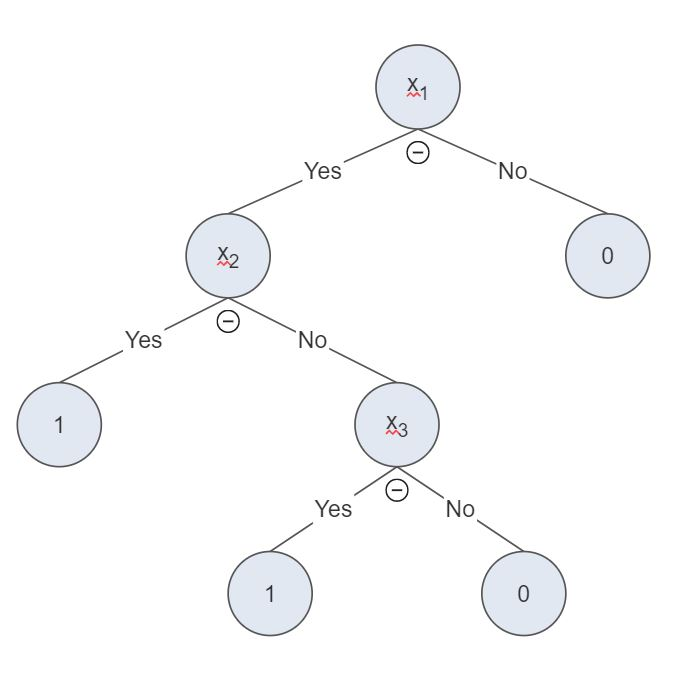
\includegraphics{figures/dec_tree_1_a}
        \end{figure}
        
        \item $(x_1\wedge x_2) \text{ xor } x_3$
        \begin{figure}[H]
            \centering
            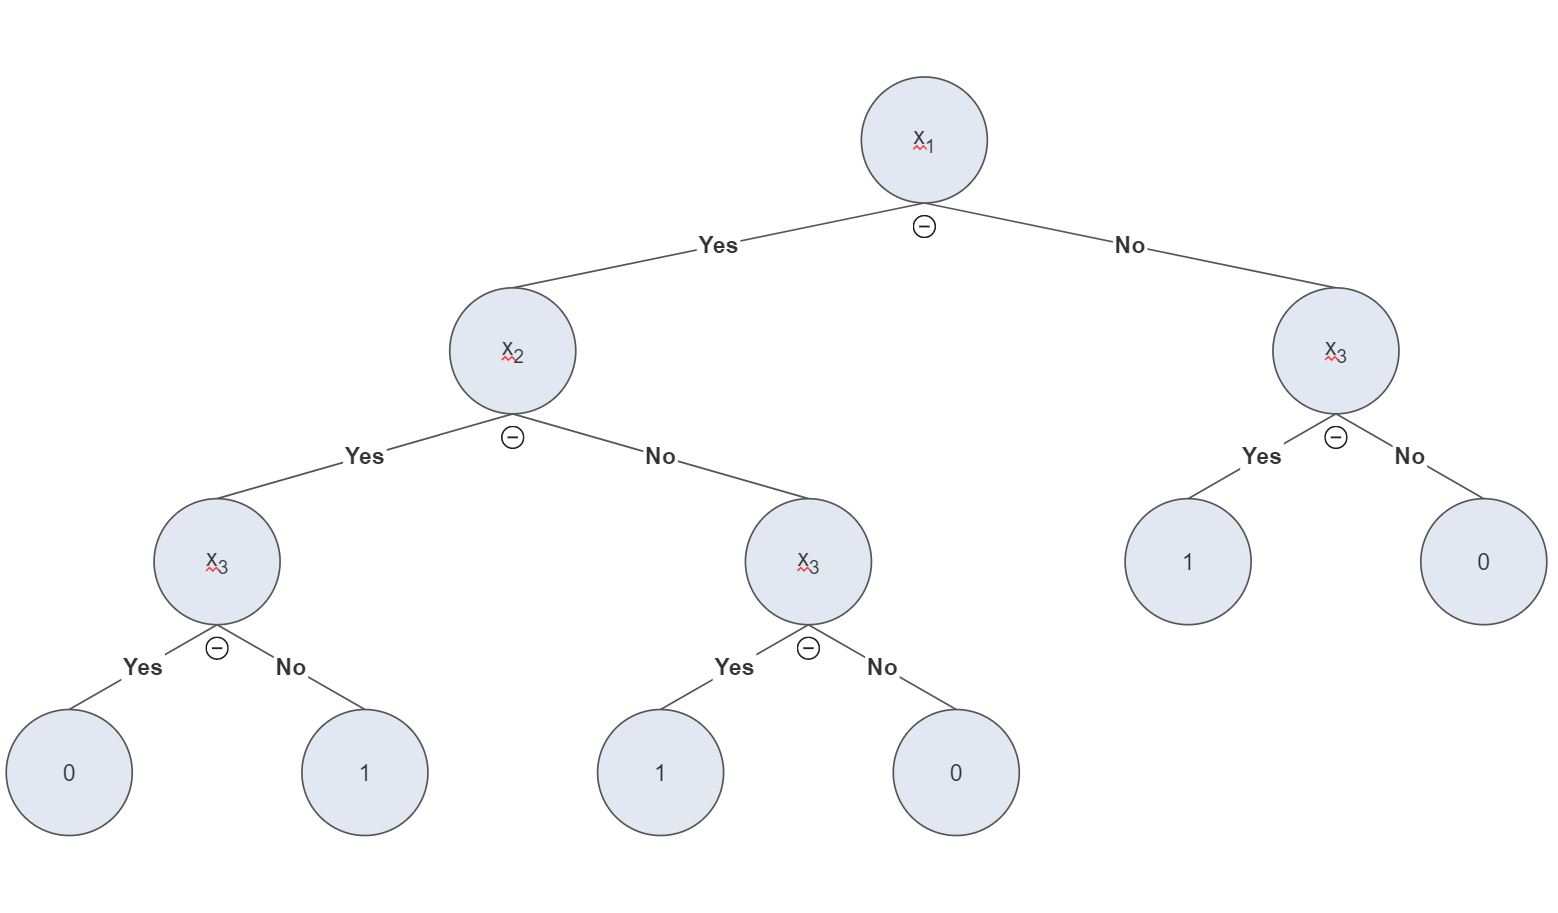
\includegraphics[width=0.7\textwidth]{figures/dec_tree_1_b}
        \end{figure}
        \item $\neg A \lor \neg B \lor \neg C \lor \neg D$
        \begin{figure}[H]
            \centering
            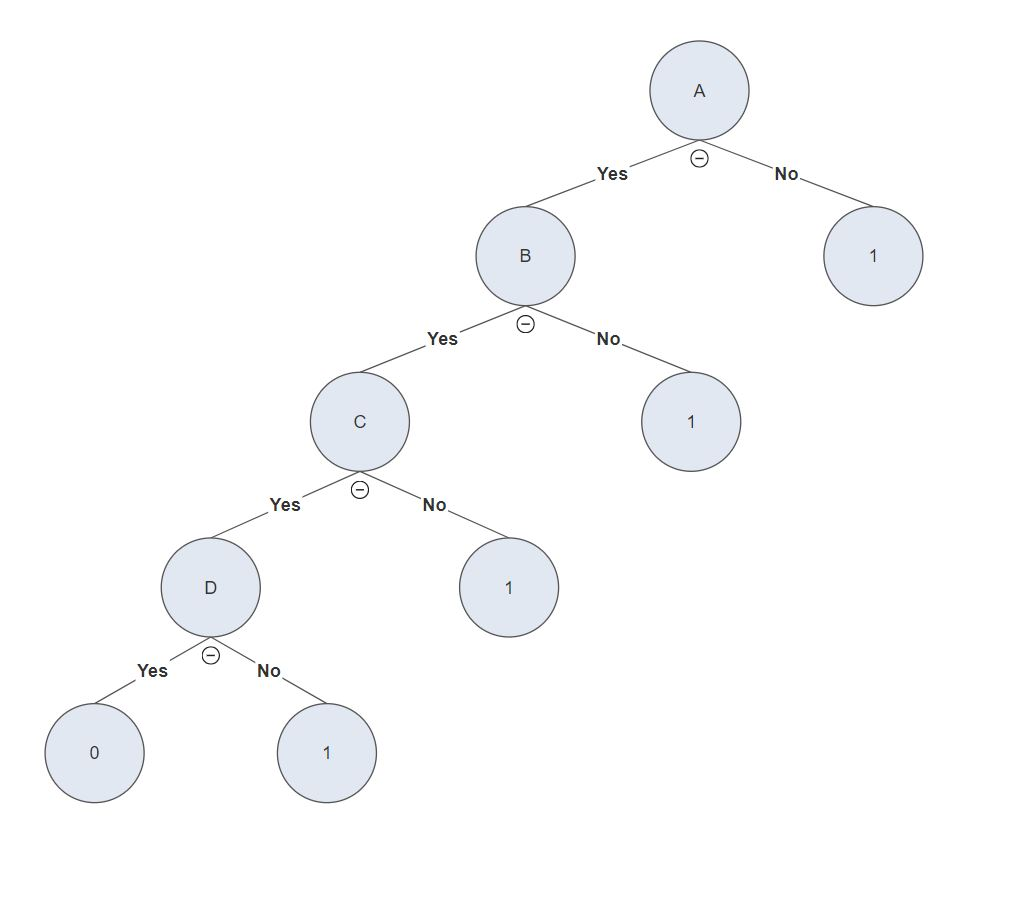
\includegraphics{figures/dec_tree_1_c}
        \end{figure}
    \end{enumerate}


\item \begin{enumerate}
    \item How many possible functions are there to map these four features to a boolean decision? How many functions are consistent with the given training dataset?
    
    
    \textbf{Answer}: Each of the features can take $2, 2, 3$ and $4$ values respectively. Thus there are  $2 \times 2 \times 3 \times 4 =2^{48}$ possible functions. Since we have observed 9 entries of the total 48 in the truth table, there are $2^{48-9} = 2^{39}$ possible functions consistent with given data.
    
    \item What is the entropy of the labels in this data?
    
    \textbf{Answer}: There are 5 points labelled ``yes" and 4 labelled ``no". 
    \begin{align*}
        entropy &= -p_{+} \log_2(p_+) - p_{-} \log_2(p_{-})\\ 
                &= -\frac{5}{9} \log_2\frac{5}{9} - \frac{4}{9} \log_2\frac{4}{9}\\
                &= 0.9911
    \end{align*}
    
    \item What is the information gain of each of the features?
    
    \textbf{Answer}: 
    \begin{table}[H]
    \centering
        \begin{tabular}{|l|ccccc|c|}
            \hline
            Feature & Value & Invade=Yes & Invade=No & Fraction of data & Entropy $\times$ fraction & Info gain \\ \hline
            \multirow{2}{*}{Technology} & Yes & 4/6 & 2/6 & 6/9 & 0.612 & \multirow{2}{*}{0.073}\\
             & No & 1/3 & 2/3 & 3/9 & 0.306 & \\ \hline
            \multirow{2}{*}{Environment} & Yes & 4/5 & 1/5 & 5/9 & 0.401 & \multirow{2}{*}{0.229}\\
             & No & 1/4 & 3/4 & 4/9 & 0.361 & \\ \hline
            \textbf{\multirow{3}{*}{Human}} & Not care & 4/4 & 0/4 & 4/9 & 0.000 & \textbf{\multirow{2}{*}{0.6305}}\\
             & Like & 1/4 & 3/4 & 4/9 & 0.361 & \\
             & Hate & 0/1 & 1/1 & 1/9 & 0.000 & \\ \hline
            \multirow{4}{*}{Distance} & 1 & 1/2 & 1/2 & 2/9 & 0.222 & \multirow{4}{*}{0.046}\\
             & 2 & 1/1 & 0/1 & 1/9 & 0.111 & \\
             & 3 & 2/3 & 1/3 & 3/9 & 0.306 & \\
             & 4 & 1/3 & 2/3 & 3/9 & 0.306 & \\ \hline
        \end{tabular}
    \end{table}
    \item Which attribute will you use to construct the root of the tree using the ID3 algorithm?
    
    \textbf{Answer}: Since {\em Human} attribute has the highest information gain, we use it to create the root node for the ID3 algorithm
    
    \item Using the root that you selected in the previous question, construct a decision tree that represents the data.
    
    \textbf{Answer}:
    
    \begin{figure}[H]
        \centering
        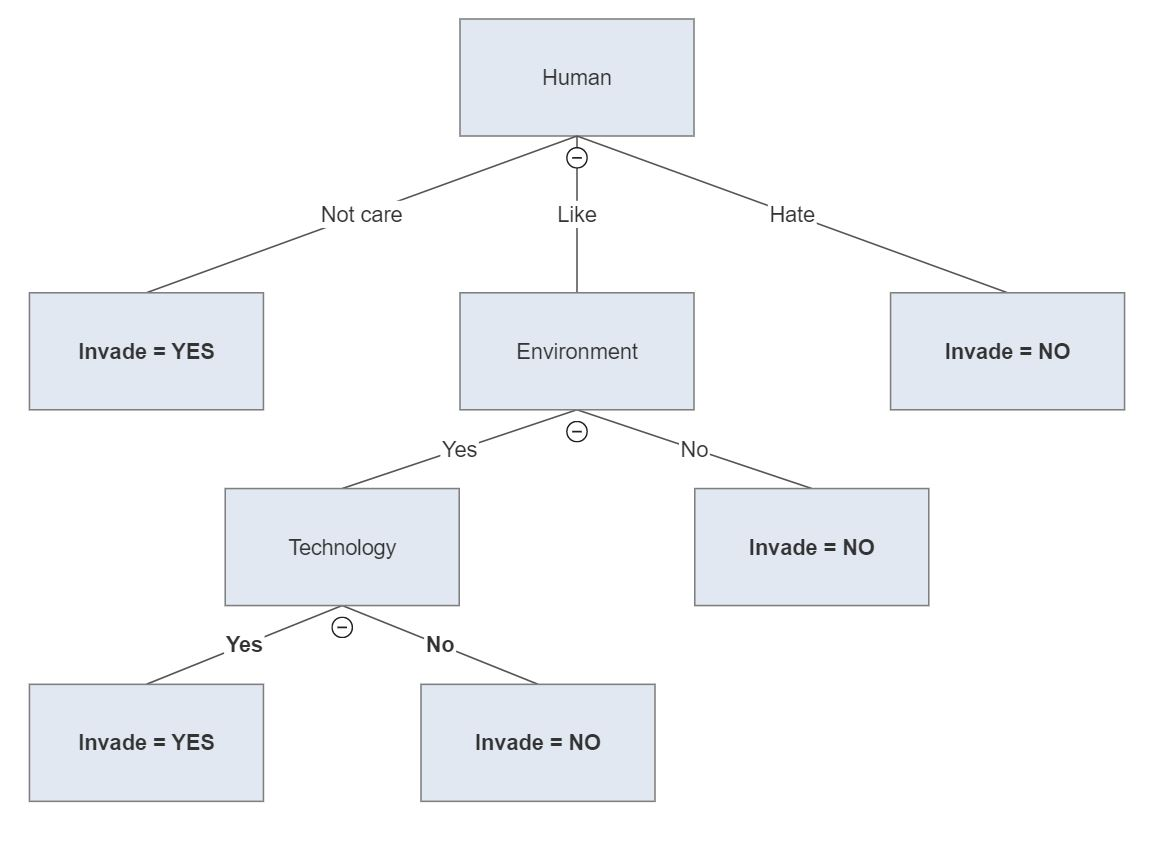
\includegraphics{figures/dec_tree_2_e.jpg}
    \end{figure}
    
    \item Suppose you are given three more examples. Use your decision tree to predict the label for each example. Also report the accuracy of the classifier that you have learned.
    
    \textbf{Answer}: 
    \begin{table}[h]
        \centering
        \begin{tabular}{cccc|c|c}
        \hline
        Technology & Environment & Human & Distance & Invade? & Prediction \\ \hline
        Yes        & Yes         & Like  & 2        & No      &  Yes \\
        No         & No          & Hate  & 3        & No      &  No  \\
        Yes        & Yes         & Lkie  & 4        & Yes     &  Yes \\ \hline
        \end{tabular}
    \end{table}
    The prediction matches 2/3 of the ground truth, hence accuracy is 67.7\%.
\end{enumerate}

\item 
\begin{enumerate}
    \item Using the $MajorityError$ measure, calculate the information gain for the four features respectively. Use 3 significant digits.
    
    \textbf{Answer}: The majority error at the root node is $1 - 5/9 = 0.444$.  
    
    \begin{table}[H]
    \centering
        \begin{tabular}{|l|ccccc|c|}
            \hline
            Feature & Value & Invade=Yes & Invade=No & Fraction of data & Majority Error $\times$ fraction & Info gain \\ \hline
            \multirow{2}{*}{Technology} & Yes & 4/6 & 2/6 & 6/9 & 0.222 & \multirow{2}{*}{0.111}\\
             & No & 1/3 & 2/3 & 3/9 & 0.111 & \\ \hline
            \multirow{2}{*}{Environment} & Yes & 4/5 & 1/5 & 5/9 & 0.111 & \multirow{2}{*}{0.222}\\
             & No & 1/4 & 3/4 & 4/9 & 0.111 & \\ \hline
            \textbf{\multirow{3}{*}{Human}} & Not care & 4/4 & 0/4 & 4/9 & 0.000 & \textbf{\multirow{2}{*}{0.333}}\\
             & Like & 1/4 & 3/4 & 4/9 & 0.111 & \\
             & Hate & 0/1 & 1/1 & 1/9 & 0.000 & \\ \hline
            \multirow{4}{*}{Distance} & 1 & 1/2 & 1/2 & 2/9 & 0.111 & \multirow{4}{*}{0.111}\\
             & 2 & 1/1 & 0/1 & 1/9 & 0.000 & \\
             & 3 & 2/3 & 1/3 & 3/9 & 0.111 & \\
             & 4 & 1/3 & 2/3 & 3/9 & 0.111 & \\ \hline
        \end{tabular}
    \end{table}
    
    \item According to your results in the last question, which attribute should be the root for the decision tree? Do these two measures (entropy and majority error) lead to the same tree?
    
    \textbf{Answer}: The highest information gain is obtained for {\em Human} attribute, hence this should be chosen as the root for the decision tree.
    Yes, both the measures lead to the same tree. Though the exact values of information gain are different for majority error and entropy, the relation between value is still same.
\end{enumerate}
\end{enumerate}
\section{Linear Classifier}
\begin{enumerate}
    \item Write a linear classifier that correctly classifies the given dataset.
    
    \textbf{Answer}: Assume that the linear classifier has weights $w_1, w_2, w_3, w_4$ and bias $b$. Substituting the datapoints in the equation for the linear classifier we get:
    \begin{align*}
        w_1 + w_3 + w_4 + b \geq 0 \\
        w_2 + w_4 + b \geq 0 \\
        w_3 + b < 0 \\
    \end{align*}
    By inspection, we find that $w_1 = w_2 = w_3$, $b = -1$ and $w_4 = 1$, all the three inequalities above are satisfied.
    
    So a linear classifier for the given data is $\textbf{w} = [0, 0, 0, 1]$, $b = -1$
    
    \item Suppose the dataset below is an extension of the above dataset. Check if your classifier from the previous question correctly classifies the dataset. Report its accuracy.

        \begin{table}[h]
        \centering
        \begin{tabular}{cccc|c|c}
            x1 & x2 & x3 & x4 & o & $sgn(\mathbf{w^Tx} + b)$ \\ \hline
            0  & 0  & 0  & 1  & 1 & 1 \\
            0  & 0  & 1  & 1  & 1 & 1 \\
            0  & 0  & 0  & 0  & -1 & -1\\
            1  & 0  & 1  & 0  & 1 & -1 \\
            1  & 1  & 0  & 0  & 1 & -1 \\
            1  & 1  & 1  & 1  & 1 & 1 \\
            1  & 1  & 1  & 0  & 1 & -1 \\
        \end{tabular}
        \end{table}
    The linear classifier given correctly classifies 3 of the 7 given inputs. Hence its accuracy is approximately 42.7\%.
    
    \item Given the remaining missing data points of the above dataset in the table below, find a linear classifier that correctly classifies the whole dataset (all three tables together)
    
    \textbf{Answer}:
    
    \begin{table}[h]
            \centering
            \begin{tabular}{cccc|c}
            $x_1$ & $x_2$ & $x_3$ & $x_4$ & $o$  \\ \hline
            1  & 0  & 1  & 1  & 1  \\
            0  & 1  & 0  & 1  & 1  \\
            0  & 0  & 1  & 0  & -1 \\
            0  & 0  & 0  & 1  & 1  \\
            0  & 0  & 1  & 1  & 1  \\
            0  & 0  & 0  & 0  & -1 \\
            1  & 0  & 1  & 0  & 1  \\
            1  & 1  & 0  & 0  & 1  \\
            1  & 1  & 1  & 1  & 1  \\
            1  & 1  & 1  & 0  & 1  \\
            0  & 1  & 0  & 0  & -1 \\
            0  & 1  & 1  & 0  & -1 \\
            0  & 1  & 1  & 1  & 1  \\
            1  & 0  & 0  & 0  & 1  \\
            1  & 0  & 0  & 1  & 1  \\
            1  & 1  & 0  & 1  & 1  \\
            \end{tabular}
        \end{table}
        
    The complete truth table is given below. All features and target values are boolean. We assume that our linear classifier is a manifestation of a boolean function of $\{x_!, x_2, x_3, x_4\}$. Looking at all rows where the output is 1 (the normal form of rows with 0 leads to $\lor$ with zero, which does not factor in the final expression), we get the following disjunctive normal form:
    \begin{align*}
        (x_1 \land \lnot x_2 \land x_3 \land x_4) \lor \\
        (\lnot x_1 \land x_2 \land \lnot x_3 \land x_4) \lor \\
        (\lnot x_1 \land \lnot x_2 \land x_3 \lnot \land x_4) \lor \\
        (\lnot x_1 \land \lnot x_2 \land x_3 \land x_4) \lor \\
        (x_1 \land \lnot x_2 \land x_3 \land \lnot x_4) \lor \\
        (x_1 \land x_2 \land \lnot x_3 \land \lnot x_4) \lor \\
        (x_1 \land x_2 \land x_3 \land x_4) \lor \\
        (x_1 \land x_2 \land x_3 \land \lnot x_4) \lor \\
        (\lnot x_1 \land x_2 \land x_3 \land x_4) \lor \\
        (x_1 \land \lnot x_2 \land \lnot x_3 \land \lnot x_4) \lor \\
        (x_1 \land \lnot x_2 \land \lnot x_3 \land x_4) \lor \\
        (x_1 \land x_2 \land \lnot x_3 \land x_4) \lor 
    \end{align*}
    Using $(x \land y) \lor (x \land \lnot y) = x$, we simplify the above expression repeatedly.
    
    This simplification yields a final expression of $\mathbf{x_1 \lor x_4}$. (The same simplification could be achieved using Karnaugh maps as well).
    
    The corresponding linear classifier for this is 
    $\mathbf{w} = [1, 0, 0, 1]$ and $b = 0$. 
    
\end{enumerate}

\section{Experiments}
\begin{enumerate}
    \item \textbf{Implementation}
    \begin{enumerate}
        \item Discuss what approaches or choices you had to make during the implementation of decision tree.
        
        \textbf{Answer}: The choice of implementation language was Python (3.5) for me. The implementation had the following stages:
        \begin{itemize}
            \item Reading the dataset into a python list
            \item Converting the strings in the data to feature vectors: This was accomplished by keep a list of functions of length $d$ and then populating the \texttt{numpy} array of size \texttt{n $\times$ d} by calling each of the \texttt{d} functions on the name string, where \texttt{n} is the number of datapoints. The labels are also stored in an array of size \texttt{d} as \texttt{[1,0]}.
            \item Creating the decision tree using \textsc{ID3} algorithm: Every node in the tree is an object of class \texttt{DecisionNode}. Every \texttt{DecisionNode} object has attributes: 
            \begin{itemize}
                \item \texttt{attr\_index}: which stores which attribute this node checks for, \texttt{-1} if leaf node
                \item \texttt{prediction}: prediction if this is a leaf node, \texttt{None} otherwise
                \item \texttt{branches}: a \texttt{dict} where keys are possible attribute values for \texttt{attr\_index}, and values are the subtree returned by \textsc{ID3}. Empty dict for leaf nodes
                The tree is built by recursive calls of \textsc{ID3} as outlined in the lecture slides.
            \end{itemize}
            Conflicting inputs where the feature vector is same but labels are different are handled by setting prediction by the last conflicting example seen in the order of input data.
            \item Performing prediction from the decision tree: On the test data, we just traverse the tree based on a \texttt{attr\_index} of the current node and follow the appropriate \texttt{branch} based on attribute value. 
        \end{itemize}
        \item Suggest at least 4 other features you could have extracted from this dataset.
        
        \textbf{Answer}: More features could be:
        \begin{itemize}
            \item Whether the ASCII sum of characters in the name is even?
            \item If the absolute difference in lengths of first and last name is less than 4? 
            \item If the number of distinct characters in name is greater than 10?
            \item If the number of distinct vowels is more than 3?
        \end{itemize}
        \item Report the error of your decision tree on the \textbf{Dataset/training.data} file.
        
        \textbf{Answer}: 91.4\%
        
        \item Report the error of your decision tree on the \textbf{Dataset/test.data} file.
        
        \textbf{Answer}: 92.8\%
        
        \item Report the maximum depth of your decision tree.
        
        \textbf{Answer}: 23 (due to 23 features, full grown tree)
    \end{enumerate}
    \item \textbf{Limiting Depth}
        \begin{enumerate}
            \item Run 4-fold cross-validation using the specified files.
            Experiment with depths in the set $\{1,2,3,4,5,10,15,20\}$, reporting the cross-validation accuracy and standard deviation for each depth. Explicity specify which depth should be chosen as the best, and explain why.
            
            \textbf{Answer}: A depth of 5 works best as observed by the 4-fold cross validation performed on the training data. This also makes intuitive sense, very deep trees tend t overfit the training data, restricting the depth forces the tree to generalize within a constrain of limited depth and can be seen as form of regularization.
            \item Using the depth with the greatest cross-validation accuracy from your experiments: train your decision tree on the \textbf{Dataset/training.data} file. Report the accuracy of your decision tree on the \textbf{Dataset/test.data} file.
            
            \textbf{Answer}: 93.03\%
            \item Discuss the performance of the depth limited tree as compared to the full decision tree. Do you think limiting depth is a good idea? Why?
            
            \textbf{Answer}: Accuracy = 91.89\%.
            
            Limiting depth is indeed a good idea. Very deep trees, though having more expressive power (they can represent boolean functions of length proportional to the depth of the tree), but this also leads to the tree `memorizing' the labels of the input, and hence is highly likely to overfit the training data. From the cross validation table in the code, we see that increasing depth first gives rise to increase in accuracy but after a certain depth the accuracy starts to drop.
        \end{enumerate}
\end{enumerate}

\section{Decision Lists}


Using the hint, we try to find a weight vector $\mathbf{w}$ and a bias term $b$ that is equivalent to the 1-decision list. Let $\mathbf{w}^T = [w_1, w_2,\ldots, w_n]$ be the linear classifier for a 1-decision list of length $n$. We also replace each negated variable $\lnot x_i$ by $z_i = \lnot x_i$. The boolean vector is $\mathbf{x} = [x_1, x_2, \ldots, z_i, \ldots, x_n]$. Hence the linear classifier is given by $sgn(\mathbf{w^Tx} + b)$. We modify $sgn$ function in an equivalent way for the convenience of proof(this definition allows us to use $b=0$).
\begin{align*}
    sgn(x) =  \begin{cases} 
                1 & x > 0 \\
                0 & x\leq 0
            \end{cases}
\end{align*}

\textbf{Observation}: If the first node evaluates to false, the entire decision list returns false. This means that $w_1$ should ``dominate" all $w_i, i \neq 1$. If $x_1$ evaluates to \textsc{TRUE}, we can follow the same process with $x_2$ as the starting node of the decision list. This idea of recursively evaluating decision lists, and the notion that the starting weight in each recursive call should ``dominate" all other weights leads us to conclude that $w_1, w_2, \ldots, w_n$ should be sorted in decreasing order and the notion of ``domination" gives the conclusion that $w_1 \geq \sum_{i=2}^{n} w_i$.\\

\textbf{Claim}: $w_i = 2^{n-i}$ and $b = 0$ gives a linear classifier for a $n$ length decision list defined as above. \\

\textbf{Inductive proof}: We prove by induction on length $n$ of decision list.
\begin{itemize}
    \item \textit{Base case} $n = 1$: $\mathbf{w} = [w_1] = [2]$. Holds trivially.
    \item \textit{Inductive case}. Let's say the $w = [2^{n-1}, 2^{n-2}, \ldots, 2^1]$ is a correct linear classifier for an $n-1$ length 1-decision list  $x = [x_2, x_3, \ldots, x_n]$. Consider the $n$ length decision list $x = [x_1, x_2, \ldots, x_n]$. There are two cases for possible values of $x_1$.
    \begin{itemize}
        \item{$x_1 = $ \textsc{FALSE}}: In this case the evaluation of decision list just calls the $n-1$ length decision list, and it's correctness is given by the inductive hypothesis.
        \item{$x_1 = $ \textsc{TRUE}}: In this case, we have to show that if $w_1 \geq w_2 + w_3 \ldots w_n$ (which happens in the worst case where $x_1 = $ \textsc{TRUE} and $x_i = $ \textsc{FALSE}, $\forall i \in \{2, 3, \ldots n\}$), which is true since $2^k \geq \sum_{i=1}^{k-1}2^i$. 
    \end{itemize}
\end{itemize}
Thus the linear classifier for 1-decision list is $\mathbf{w^Tx}$, $\mathbf{w} = [2^{n}, 2^{n-1}, \ldots, 2^1], b = 0$.
\end{document}
